\documentclass{article}
\usepackage{amsmath}
\usepackage{amsthm}
\usepackage{tikz}
\usetikzlibrary{arrows}
\newcommand\independent{\protect\mathpalette{\protect\independenT}{\perp}}
\def\independenT#1#2{\mathrel{\rlap{$#1#2$}\mkern2mu{#1#2}}}
\DeclareMathOperator*{\argmin}{arg\,min}
\DeclareMathOperator*{\argmax}{arg\,max}
\newtheorem{theorem}{Theorem}
\newtheorem{mydef}{Definition}
\title{Learning Neighborhoods}
\author{Forest Gregg}
\begin{document}
\maketitle


The fundamental methodological problem of studying the neighborhood is
the fundamental methodological problem of sociological inquiry. Our
claims about what neighborhoods are or do depends upon how we carve up
the city into neighborhoods. Unless we believe we cut at the joints,
then we should not believe that we are learning about anything beyond
our own butchery.

The dangers of ecological fallacies are, by now, familiar to urban
sociologists. At least among those with a quantitative bent, we have
mostly responded by trying not to make any cuts at all--we use the
most finely grained data available and include spatial auto-regressive
terms in our statistical models. These models imply a city where one
part of the city can be very different from another, but two adjacent
blocks cannot.

However, while this approach may yield much more reliable estimates
of, say, the effect of `collective efficacy' on murder rates, this
approach does not permit allow us to estimate the effects of a thing
we call a neighborhood.

This may not be any great loss, but let's make sure we understand the
stakes. On one hand, we have a view of the city as ultimately
continuous. Near things will always have more effect than far
things. While this lacks face validity if we only consider spatial
distance, we could think of a distance as function of spatial
distance, travel distance, and social distance. With a more
sociologically realistic distance, the continuous view of the city may
be hard to visualize but seems quite possibly correct.

On the other hand, we have a view of the city as being composed to
elemental units. These are geographically contiguous areas that 1.)
share a common fate, 2.) and where there are social processes which
are discontinuous at the edges of an area. Let's call these elemental
units neighborhoods. Under this view, there is no distance function
that could restore the continuity to the city, save one that took into
account the unitary nature of neighborhoods.

Beyond the thrill of re-enacting debates between Parmenides and
Democritus, there are three reasons why we might care which of these
models of cities is true. First, if cities are truly continuous, but
we modeled them as composed then we risk ecological fallacies. If
cities are truly composed, but we treat them as continuous we will
perpetually underestimate the effects of place on our lives, because
our methods will smooth truly sharp discontinuities

Second, if we have the wrong model, either way, then we will not be
able to understand the history or predict the future of land use
across a city. We will not understand neighborhood transition. Ernest
Burgess believed he needed to know where the elemental units of city
were, which he called ecological areas, in order to understand how the
dynamism of his bid-rent model would play out in the real
city. Changes would not occur smoothly across space and time, but be
channeled, pent up, and released as economic competition worked over
the joints of the city.  If he was wrong and the city was truly
continuous, the current patterns of land use would be as predictive of
the future as a photograph of waves in the open sea.

Finally, and most parochially, sociologists have a vested interest in
a view of the world as being composed of real social categories. If we
can find that neighborhoods are real, maybe we will learn how we might
do the same for some of other favorite, but empirically battered
categories like class and status group.

Today I'd like to describe how I think we might be able to learn to
identify real neighborhoods, the elementary unit sense; how we might
convince ourselves we have actually done so, and what both might say
about how real neighborhoods originate and persist.

\section*{Subjective Sense}

Ten years ago, the clear and bright line dividing Hyde Park and
Woodlawn was the Midway, a `natural barrier' if there ever was
one. Now I ask recent arrivals in the University, and I hear more and
more often that Woodlawn begins at 63rd Street. 

Ten years ago, there was no South Campus, there was no Toyota
Institute, there was no Logan Center, there were not bright, beautiful
lights spanning the walkways, there were not security personnel at
every corner on both sides of the Midway, the UCPD's service area did
not extend down to 63rd, and there not nearly as many students living
in apartments below 60th. In the past 10 years, the area between the
60th and 63rd has become much more like Hyde Park. Recent arrivals are
responding to that. If that area seems like Hyde Park then why
shouldn't they think it's Hyde Park.

But what does it mean for an area to seem like Hyde Park or not? What
are people responding to when they perceive two adjacent places as
belonging to the same place or belonging to different place? I'm not
sure, but I think we can learn. 

To do so, I need to make following assumptions.

\begin{itemize}
\item If a person is likely to see two adjacent areas as part of
  different neighborhoods, those areas are likely to feel different to her.
\item In large part, that different feeling is in response to
  differences between the areas that another person, who did not know
  that the areas were supposed to belong to different neighborhoods,
  would notice.
\end{itemize}

In other words, I am assuming that we tend to assign different
neighborhood names to places that seem different, in ways that are
not private to individuals, and which do not solely depend upon having
learned what places belong to what neighborhoods.

Supposing that's true, then it may well be possible to learn how to
predict what areas are likely to be perceived as different
neighborhoods. We just need data on what place particular spots of the
city are claimed to belong to, data on what is going in those spots
that people might be feeling, and some admittedly complicated
statistical machinery.

\subsection*{Data}

I have a nightly updated database of geocoded Craigslist apartment
rentals, sublet, and roommate listings. For most of these listings,
the poster entered some text in a ``Specific Location'' field. With
some minimal pre-processing, we can use these data as observations of
claims that geographical points are in some neighborhood.

Using kernel density estimation, we can use this point data to
estimate a continuous probability distributions that any point in the
city will be claimed to be in any of the neighborhoods (Figure
\ref{fig:KDE}). The gray lines indicate the best guess about the
neighborhood boundaries.

\begin{figure}
\includegraphics{/home/fgregg/sweave-cache/figs/fig-KSplot.pdf}
\caption{KDE probability estimates of neighborhood claims on North Side}
\label{fig:KDE}
\end{figure}

I would like to treat this measure as a kind of `averaged neighborhood
perception.' Of course, it's biased measure of that. There are
enormous selection effects, but perhaps more troublesome is that
listers are likely to choose neighborhood claims strategically in
order to make a listing maximally desirable. I have been looking for
scientific samples of neighborhood perception that I can compare
against so as to get a sense of magnitude of the biases.

However, I think it's possible that these data, with their biases
might be good enough, and we'll have ways of checking that. 

In addition to these data about neighborhood perception, we also have
block level census data as well as a trove of unaggregated data from
the City of Chicago on the built environment, crimes, 311 reports,
zoning, and the similar. We'd like to set them in relation to each
other.

\subsubsection*{Where are the edges}
To demonstrate the general approach, let's try to make a hopefully
uncontroversial improvement to our map of average neighborhood
perception. Most of you will accept that the front of house is
typically not in one neighborhood while the back of it is another. We
would think that neighborhood boundaries are more likely to fall along
streets, and even more likely to follow a major geographic divider
like the river, a railroad embankment, or major commercial street.

If we could mathematically incorporate these beliefs into model of
neighborhood perception then, we should expect to get a more precise
estimate.

Without these beliefs, we can write down the probability for a
particular pattern of assignments of neighborhood names to $n$ blocks as
follows.

\begin{equation}
\Pr(Y)= \frac{1}{Z}\prod_i^nPr_i(\text{Name}) 
\end{equation}

where $\Pr_i(\text{Name})$ is the probability of the $i$th block being
assigned one of finite set of neighborhood names, and $Z$ is a
normalizing constant. We'll find it convenient to rewrite this as

\begin{equation}
\Pr(Y) = \frac{1}{Z}\operatorname{exp}\left(\sum_i^n\epsilon_i(\text{Name})\right) 
\end{equation}

where $\epsilon_i(\text{Name})$ is the log probability of $i$th block
being assigned one finite set of neighborhood names.

Since we have the idea that neighborhoods are contiguous areas, we might
want to encourage neighboring blocks to share the same name. We'll add
a term, $\epsilon_{i,j}$, that will discourage adjacent blocks from
having different names.

\begin{equation}
\epsilon_{i,j}(\text{Name}_i,\text{Name}_j) = \begin{cases}
  0 \quad\quad \text{Name}_i = \text{Name}_j \\
  \lambda \quad\quad \text{Name}_i \neq \text{Name}_j 
\end{cases}
\end{equation}

Except, we don't want to discourage blocks that are separated by a
major street, river, or railroad embankment to have different names,
so let's amend $\epsilon_{i,j}$.

\begin{equation}
\epsilon_{i,j}(\text{Name}_i,\text{Name}_j) = \begin{cases}
  0 \quad\quad \text{Name}_i = \text{Name}_j \\
  0 \quad\quad \text{if $i$, $j$ are separated by a barrier} \\
  \lambda \quad\quad \text{Name}_i \neq \text{Name}_j 
\end{cases}
\end{equation}


So, that our model becomes

\begin{equation}
\Pr(Y) = \frac{1}{Z}\operatorname{exp}\left(\sum_{<i j>}\epsilon_{i,j}(\text{Name}_i,\text{Name}_j) + \sum_i\epsilon_i(\text{Name}_i)\right) 
\end{equation}

Where $<i j>$ indexes all neighboring blocks.

By finding the most likely assignment of neighborhood names to blocks
within that distribution, we can get segmentation of the city seen in
Figure \ref{fig:graphcut}.


\begin{figure}
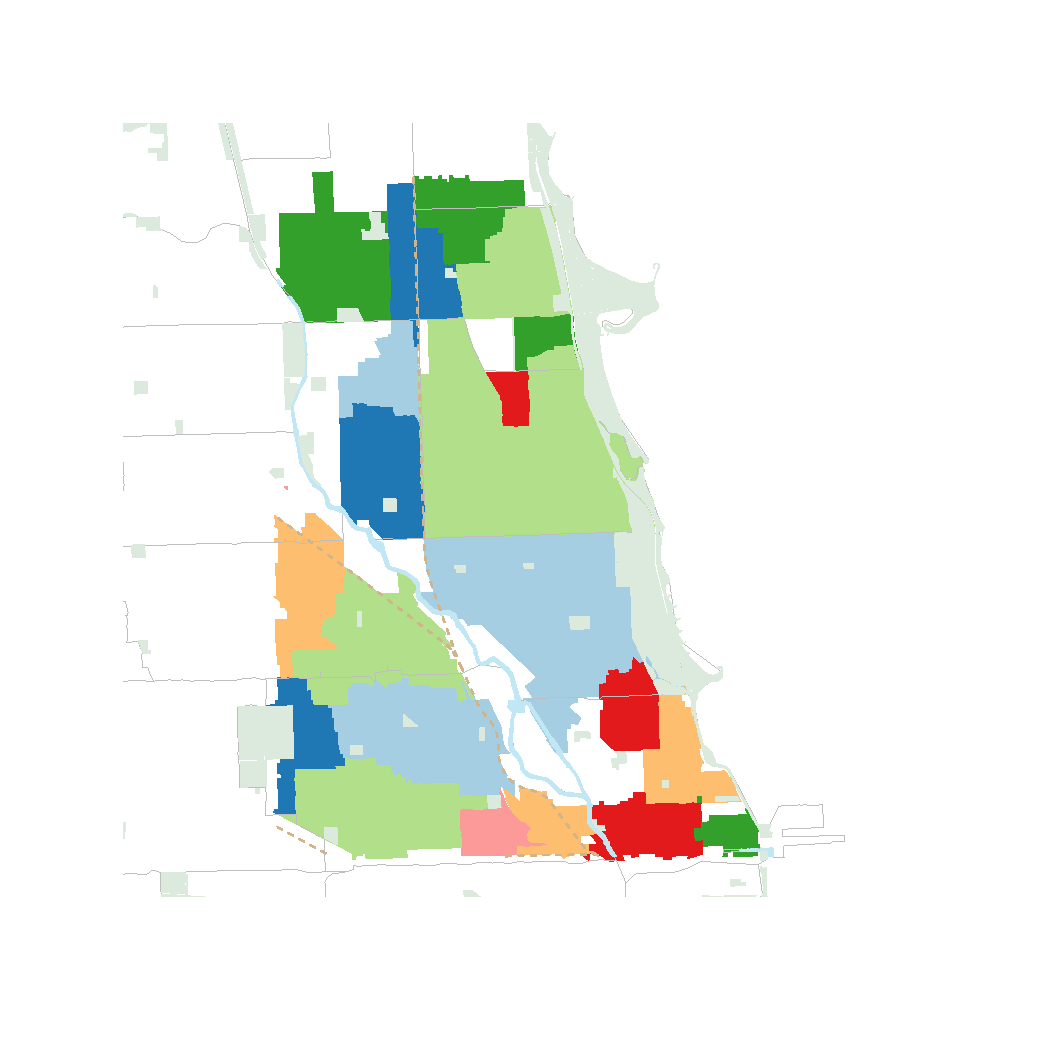
\includegraphics{respect_grid.pdf}
\caption{MAP estimate of neighborhood labels}
\label{fig:graphcut}
\end{figure}



\subsection*{Learning}
As we saw in this example, by manipulating the inter-block term,
$\epsilon_{i,j}$ we can move these neighborhood boundaries around. If
we had the right $\epsilon_{i,j}$, we could even reproduce those
neighborhood boundaries without knowing anything about people's
perceptions.

Think of $\epsilon_{i,j}$ as a kind of stress function. Depending on
its form, it adds a certain amount of stress, if two neighboring
blocks have the same name or not. If we think that stress depends upon
the nature of the two blocks, then we could approximate
$\epsilon_{i,j}$ as a linear function of inter-block differences. 

For example: 

\begin{equation}
\epsilon_{i,j}(\text{Name}_i,\text{Name}_j) = \begin{cases}
  \beta_0 + \beta_1(\text{Median Income}_i - \text{Median Income}_j)& \quad\text{Name}_i = \text{Name}_j \\
  - \beta_0 - \beta_1(\text{Median Income}_i - \text{Median Income}_j)& \quad\text{Name}_i \neq \text{Name}_j \\
\end{cases}
\end{equation}

Given a `stress' function, we can find the segmentation of the city
that minimizes that stress, which ends up being the most likely
assignment from the distribution:

\begin{equation}
\Pr(Y) = \frac{1}{Z}\operatorname{exp}\left(\sum_{<i j>}\epsilon_{i,j}(\text{Name}_i,\text{Name}_j)\right) 
\end{equation}

If we find the right function, then we can reproduce the segmentation
of the city that we derived from people's perceptions. The details of
how would take us far afield, but given a linear model of the
function, like we described above, it is possible to learn parameters
that would make some target segmentation most likely. Understanding
and setting up the machinery to do this is what I have spend most of
this quarter doing.

\section*{Validating segments}
Let's say we learned the right `stress function.' If we had that, we
would have some machinery that could read in block by block data for a
city and produce segmentations of the city that were likely to be
perceived as real areas by the residents. 

This claim is relatively easy to check. I have been collecting this
same Craigslist data for the top 50 American cities by population. The
first hurdle will be to see whether the trained model can predict
`averaged neighborhood perceptions' in out of sample cities.

Assuming that actually works, all I have demonstrated is that I can
predict how Craigslist users will segment a city. It's not nothing,
but its also not what I promised.

To show that we can use this method to find the real joints of the
city, we'll have to do something else. Right now, the most convincing
test seems to be predicting the past.

\subsection*{Palmer's primary settlements}
In abstract, Ernest Burgess's model of urban ecology predicted that
concentric circles of land use and social processes issuing from a
central business district. However, Burgess always argued that a city
was not an abstract homogeneous space, but comprised of natural areas
that would shape the configuration of zones for any particular
city. In the 1920s, he collaborated with Vivien Palmer to define these
natural areas and to test the ecological theory of urban process.

In the eight years that she studied Chicago's communities, Palmer
pushed long and hard on the problem of the how to carve up city. Her
efforts have not yet, I think, been equaled. I quote from her
dissertation.

\begin{quote}
As our natural histories accumulated we began to realize that the
ecological areas which had been defined mainly by topographic and
economic criteria did not give us the elementary territorial
groupings of the city. With our extensive research into these
ecological areas we were finding that the majority of them contained a
number of smaller territorial groupings which were often bound
together at the present time by a common shopping and commercial
center which sometimes shared other institutions. Yet these units had
other distinctive characteristics and group relationships, often
subtle yet recognized by their residents, which set them apart
from each other. So we sought to formulate some new conception which
would enable us to explain the existence of these smaller groupings
and delimit them objectively... 

A more careful examination of natural histories, of the account of the
development of the natural territorial led us to the conception of the
primary settlement areas as the unit of our research. 

As Chicago expanded outward from its embryo village of a few square
miles it grew decade by decade, and is till growing, by the addition
of small relatively isolated settlements. With an abundance of open
land always on its borders and under our present system of property
ownership, small sections usually known as subdivisions were being
placed on market for industrial , business, and home sites. As the
city grew, also, its populations was becoming increasingly
heterogeneous and and groups relatively homogeneous in nationality,
economic status, and occupational strata were becoming segregated in
each of these new primary settlements. Most of these areas developed a
local life and character. Taken together they constituted a natural
social organization of the  city which was primary and over which
many of the later forces of city growth had to work themselves over.\footnote{Palmer, Vivien Marie. 1932. ``The Primary Settlement as a
Unit of Urban Growth and Organization''. Dissertation, Chicago:
University of Chicago., p.30-33}
\end{quote}

The approach I propose allows, for segmenting the city into finer our
courser chunks. If my method is capable of finding real neighborhoods,
or real neighborhoods exist to be found, then I should be able to
recover Palmer's primary settlements.

If that's successful then I think that I will have shown that Palmer
was right, that primary settlements truly are the elements of a city,
if they still predict perceptually distinct areas 90 years later, and
that I am right that perceptually distinct areas will be elements of a
city if they are the results of patterns set 90 years ago.

\section*{Forming a field}
By now the chain of conditional successes has grown comically long,
but once again, assuming that we can build confidence that this
methods identifies real neighborhoods, what would it mean for how
real neighborhoods originate and persist. 

I think that Ms. Palmer got it about right 90 years ago. The initial
speedy development of an area endows an area with a certain
homogeneity, such that residents are likely to respond similarly to
urban processes working over the city and the given built environment
will be similarly valued or disvalued in various states of the real
estate market. The only thing missing from Palmer is the recognition
of self-reinforcing aspect of that homogeneity. Historic greystones
are more attractive when surrounded by other greystones then when they
are surrounded by vacant lots, and it's easier for an immigrant to
move into a majority immigrant area. 

When local states make those states more likely, we often call this a
field effect. The classic example is magnetism, where the local
alignment of polarized molecules can increases the field strength that
encourages the polarization of other molecules and helps keep
molecules polarized. The statistical models used to describe magnetism
are exactly of the form that I am proposing to model neighborhood perception. 
\end{document}